\documentclass[11pt,usenames,dvipsnames,
hyperref={pdfencoding=auto,psdextra}]{beamer}
\def\showTODOs{}


\usepackage{gensymb}

\newcommand*{\listsofb}[1]{\mathcal{L} (#1)}
\newcommand*{\listsof}{\mathcal{L}~}

\newcommand{\None}{\emptyset}
\newcommand{\Some}[1]{\degree\kern-0.5ex#1}
\newcommand{\lnil}{\ensuremath{[]}}

\newcommand*{\match}{\textbf{match}~}
\newcommand*{\withl}{\textbf{[}~}
\newcommand*{\withr}{~\textbf{]}}
\newcommand*{\withm}{\quad\textbf{|}\quad}
\newcommand*{\llet}{\textbf{let}~}
\newcommand*{\lin}{\textbf{in}~}
\newcommand{\ITE}[3]{\textbf{if}~{#1}~\textbf{then}~{#2}~\textbf{else}~{#3}}

\newcommand{\Type}{\mathbb{T}}
\newcommand{\Prop}{\mathbb{P}}
\newcommand{\bool}{\mathbb{B}}
\newcommand{\btrue}{\mathsf{T}}
\newcommand{\bfalse}{\mathsf{F}}
\newcommand{\andb}{\&\&}
\newcommand{\orb}{||}
\newcommand{\notb}{!}
\newcommand{\nat}{\mathbb{N}}
\newcommand{\natS}{1 + }
\newcommand{\length}[1]{|#1|}

\newcommand{\con}{\mathop{{+}\!\!\!{+}}}
\newcommand{\rev}{\mathsf{rev}}
\newcommand{\opt}[1]{\mathcal{O}{#1}}

\newcommand{\eqb}[2]{#1\overset{?}{=}#2}

\usepackage[english]{babel}
\usepackage{lipsum}
\usepackage{mathtools}
\usepackage{pifont}
\usepackage{wasysym}
\usepackage{booktabs}
\usepackage{multirow}
\usepackage[absolute,overlay]{textpos}
\usepackage{proof}
\usepackage{amsmath}
%\usepackage[utf8]{inputenc}
\usepackage{listings}
\usepackage{tikz}
\usetikzlibrary{automata,trees,calc,arrows.meta,positioning,decorations.pathreplacing,bending,shapes.geometric, intersections, hobby}
\usetheme{Berlin}
\usepackage{cite}
\usepackage{cancel}
\usepackage{xsavebox}
\usepackage[normalem]{ulem}
\usepackage{array}
%\usepackage{wasysym}
\usepackage{stmaryrd}
\usepackage{pgfplots}
\usepackage{ifthen}


\pgfplotsset{compat=1.16}

%some nicer colour scheme
\definecolor{craneorange}{RGB}{237, 142, 26}
\definecolor{craneblue}{RGB}{0,0,0}

\setbeamercolor{structure}{fg=craneblue}

\setbeamercolor{palette primary}{fg=craneblue,bg=craneorange!70}
\setbeamercolor{palette secondary}{fg=craneblue,bg=craneorange!80}
\setbeamercolor{palette tertiary}{fg=craneblue,bg=craneorange!90}
\setbeamercolor{palette quaternary}{fg=craneblue,bg=craneorange}

\setbeamercolor{titlelike}{parent=palette quaternary}

\setbeamercolor{block title}{fg=craneblue,bg=craneorange}
\setbeamercolor{block title alerted}{use=alerted text,fg=craneblue,bg=alerted text.fg!75!bg}
\setbeamercolor{block title example}{use=example text,fg=craneblue,bg=example text.fg!75!bg}

\setbeamercolor{block body}{parent=normal text,use=block title,bg=block title.bg!15!bg}
\setbeamercolor{block body alerted}{parent=normal text,use=block title alerted,bg=block title alerted.bg!15!bg}
\setbeamercolor{block body example}{parent=normal text,use=block title example,bg=block title example.bg!15!bg}

\setbeamercolor{sidebar}{bg=craneorange!70}

\setbeamercolor{palette sidebar primary}{fg=craneblue}
\setbeamercolor{palette sidebar secondary}{fg=craneblue!75}
\setbeamercolor{palette sidebar tertiary}{fg=craneblue!75}
\setbeamercolor{palette sidebar quaternary}{fg=craneblue}

\setbeamercolor*{separation line}{}
\setbeamercolor*{fine separation line}{}

\setbeamercolor{frametitle}{bg=white}

%no frame numbering when using framebreaks
\setbeamertemplate{frametitle continuation}{}

%no total frame number
\setbeamertemplate{footline}{% 
  \hfill% 
  \usebeamercolor[fg]{page number in head/foot}% 
  \usebeamerfont{page number in head/foot}% 
  \insertframenumber%
  %\,/\,\inserttotalframenumber
  \kern1em\vskip2pt% 
}

%no subsection line
\setbeamertemplate{headline}
{%
  \begin{beamercolorbox}[colsep=1.5pt]{upper separation line head}
  \end{beamercolorbox}
  \begin{beamercolorbox}{section in head/foot}
    \vskip0pt\insertnavigation{\paperwidth}\vskip3pt
  \end{beamercolorbox}%
  \begin{beamercolorbox}[colsep=1.5pt]{lower separation line head}
  \end{beamercolorbox}
}

%highlight colours to be used throughout the presentation
\newcommand{\highlight}[1]{\color{blue}#1\color{black}}
\newcommand{\colorHOne}{\color{red}}
\newcommand{\colorHThree}{\color{violet}}
\newcommand{\colorHTwo}{\color{blue}}
\newcommand{\colorHFour}{\color{green}}

\newcommand{\colorTikzA}{red}
\newcommand{\colorTikzB}{cyan}
\newcommand{\colorTikzC}{blue}
\newcommand{\colorTikzD}{green}
\newcommand{\colorTikzE}{violet}

%don't count the title page
\let\otp\titlepage
\renewcommand{\titlepage}{\otp\addtocounter{framenumber}{-1}}

%a hide on=... option for tikz elements, where the usual ranges allowed by \only are allowed for ...
\tikzset{hide on/.code={\only<#1>{\pgfkeysalso{white}}}}

%don't want those nasty navigation symbols
\beamertemplatenavigationsymbolsempty


\newenvironment{tightcenter}{%
  \setlength\topsep{0pt}
  \setlength\parskip{0pt}
  \begin{center}
    }{%
  \end{center}
}

%table column types for fixed width
\newcolumntype{L}[1]{>{\raggedright\let\newline\\\arraybackslash\hspace{0pt}}m{#1}}
\newcolumntype{C}[1]{>{\centering\let\newline\\\arraybackslash\hspace{0pt}}m{#1}}
\newcolumntype{R}[1]{>{\raggedleft\let\newline\\\arraybackslash\hspace{0pt}}m{#1}}

\newcommand{\TODO}[1]{\ifthenelse{\isundefined{\showTODOs}}{}{\colorbox{red}{\LARGE TODO}:#1}}


%math stuff
\newcommand*{\Eq}{\text{Eq}}
\newcommand*{\N}{\mathbb{N}}
\newcommand*{\R}{\mathbb{R}}
\newcommand*{\Reach}{\text{Reach}}
\newcommand*{\norm}[1]{\left\lVert#1\right\rVert}
\newcommand*{\diff}{\text{d}}
\newcount\colveccount
\newcommand*\colvec[1]{
  \global\colveccount#1
  \begin{pmatrix}
    \colvecnext
  }
  \def\colvecnext#1{
    #1
    \global\advance\colveccount-1
    \ifnum\colveccount>0
      \\
      \expandafter\colvecnext
    \else
    \end{pmatrix}
  \fi
}


%prevent backup slides from appearing in the header
\makeatletter
\let\beamer@writeslidentry@miniframeson=\beamer@writeslidentry%
\def\beamer@writeslidentry@miniframesoff{%
  \expandafter\beamer@ifempty\expandafter{\beamer@framestartpage}{}% does not happen normally
  {%else
    % removed \addtocontents commands
    \clearpage\beamer@notesactions%
  }
}
\newcommand*{\miniframeson}{\let\beamer@writeslidentry=\beamer@writeslidentry@miniframeson}
\newcommand*{\miniframesoff}{\let\beamer@writeslidentry=\beamer@writeslidentry@miniframesoff}
\makeatother


%footnote without marker, for images
\newcommand\blfootnote[1]{%
  \begingroup
  \renewcommand\thefootnote{}\footnote{#1}%
  \addtocounter{footnote}{-1}%
  \endgroup
}

\newcommand{\bnfmid}{~\mid~}

\newcommand*{\PR}{\textbf{PR}}
\newcommand*{\sat}{\textbf{SAT}}
\newcommand*{\gennp}{\textbf{TMGenNP}}
\newcommand{\fsat}{\textbf{FSAT}}
\newcommand{\NP}{\textsf{NP}}

\newcolumntype{C}{>{$}c<{$}}
\newcommand{\rewwin}[2]{
  \begin{tabular}{C|C|C}
    #1 \\ 
    \midrule #2
  \end{tabular}
}

\newcommand{\trewwin}[6]{
  \begin{tikzpicture}
    \draw[thick] (0, 0) -- (2.25, 0);
    \draw (0.75, -0.75) -- (0.75, 0.75);
    \draw (1.5, -0.75) -- (1.5, 0.75);
    \node at (0.375, 0.375) {\ensuremath{#1}};
    \node at (0.375, -0.375) {\ensuremath{#4}};
    \node at (1.125, 0.375) {\ensuremath{#2}};
    \node at (1.125, -0.375) {\ensuremath{#5}};
    \node at (1.875, 0.375) {\ensuremath{#3}};
    \node at (1.875, -0.375) {\ensuremath{#6}};
  \end{tikzpicture}
}

%workaround so that polarities on blanks have the same height as on other symbols
\newcommand*{\TallestContent}{\ensuremath{b \sigma_1}}% <-- This should be the tallest content

\newcommand{\polneg}[1]{\overleftarrow{#1\vphantom{\TallestContent}}}
\newcommand{\polpos}[1]{\overrightarrow{#1\vphantom{\TallestContent}}}
\newcommand{\polneut}[1]{\overline{#1\vphantom{\TallestContent}}}

\newcommand{\reprt}[1]{\ensuremath{\sim_t^{#1}}}
\newcommand{\reprtt}[2]{\ensuremath{\sim_t^{(#1, #2)}}}
\newcommand{\reprc}{\ensuremath{\sim_c}}



\newcommand{\strent}{\rightsquigarrow}
\newcommand{\constrent}{\overset{!}{\rightsquigarrow}}
\newcommand{\Rfinal}{R_{\text{final}}}

\newcommand{\blank}{\textbf{\textvisiblespace}}


\title{Towards a Formal Proof of the Cook-Levin Theorem}

\institute{Saarland University}
\date{15 April 2020\\[1ex]Final Bachelor Talk}
\author{Lennard Gäher\\[1mm] {\small{Advisor: Fabian Kunze}\\ \small{Supervisor: Prof.\ Smolka}}}

\begin{document}
\begin{frame}[plain]
  \titlepage
\end{frame}

\section{Introduction}
\begin{frame}{Timeline}
  \begin{tikzpicture}[overlay,remember picture]
    \node[minimum width=\paperwidth,minimum height =\paperheight,anchor=north west] (a) {};
    \draw[thick,->] ($(current page.north east)!0.5!(current page.north west) + (0, -0.57)$) -- ($(current page.south west)!0.5!(current page.south east) + (0, 1)$);
  \end{tikzpicture}
  \only<4->{\frametitle{Timeline: Mechanisation}}

  \setlength{\TPHorizModule}{\textwidth}
  \setlength{\TPVertModule}{\textwidth}
  \begin{textblock}{0.5} (0.62, 0.15)
    \small
    \textbf{1965:} time/space complexity, hierarchy theorems, \ldots

    \emph{On the Computational Complexity of Algorithms}

    Hartmanis and Stearns\\
    \onslide<4->{
      $~$\\
      {
        \colorHTwo{}
        mechanisation without reference to concrete model (Matita)~\cite{asperti:reverse_complexity}
      }
    }
  \end{textblock}

    \begin{textblock}{0.5} (0.05, 0.45)
      \onslide<2->{
        \small 
        \textbf{1971:} Cook-Levin Theorem

        \emph{The Complexity of Theorem-Proving Procedures}

        Stephen A.\ Cook\\
        \onslide<5->{
          $~$\\
          { 
            \colorHTwo{}
            verified construction without connection to computational model (ACL2)~\cite{gamboa:cook}
          }
        }
      }
    \end{textblock}

    \begin{textblock}{0.5} (0.62, 0.6)
    \onslide<3->{
        \small
        \textbf{1972:} Karp's 21 NP-complete problems

        \emph{Reducibility Among Combinatorial Problems}

        Richard M.\ Karp
      }
    \end{textblock}
\end{frame}

\begin{frame}{What makes mechanisations hard?}
  Prevalent computational model: Turing machines 
  $~$\\[5ex]
  \begin{quote}
    Turing machines as model of computation are inherently infeasible for the formalisation of any computability- or complexity-theoretic result
  \end{quote}
  \raggedleft{} \cite{ForsterEtAl:2019:VerifiedTMs}

  \raggedright{}
  Here: use $\lambda$-calculus L

  Supported by: 
  \begin{itemize}
    \item Reasonability~\cite{ForsterKunzeRoth:2019:wcbv-Reasonable}
    \item Extraction mechanism in Coq~\cite{ForsterKunze:2019:Certifying-extraction}
  \end{itemize}
\end{frame}

\begin{frame}{The call-by-value $\lambda$-calculus L}
  \TODO{superficial stuff as a quick refresher which is needed to understand why it would be hard to directly encode L in SAT}
  \TODO{basic definitions of complexity theory: superficial, basically the same as for TMs}
\end{frame}

\newcommand{\SAT}{\textbf{SAT}}
\begin{frame}{The Cook-Levin Theorem}
  \begin{center}
    \SAT{} is \NP{}-complete. 
  \end{center}
  \vspace{2ex}
  \begin{block}{SAT}
    Given a Boolean formula in conjunctive normal form, does there exist a satisfying assignment?
  \end{block}
  \vspace{1ex}
  Idea: encode computation as Boolean formula\\[2ex]

  \onslide<-1>{L: non-local computations, too high-level \frownie{}}
  \begin{center}
  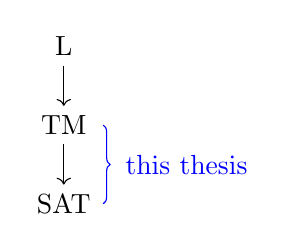
\begin{tikzpicture}
    \node (L) at (0, 3) {L};
    \node (TM) at (0, 2) {TM};
    \node (SAT) at (0, 1) {SAT};
    \draw[->] (L) -- (TM);
    \draw[->] (TM) -- (SAT);

    \draw[decorate, decoration={brace}, color=\colorTikzC] (0.5, 2) -- (0.5, 1) node[midway, xshift=1.0cm] {\colorHTwo{} this thesis};
  \end{tikzpicture}
\end{center}
\end{frame}

\begin{frame}{Generic Problem for Turing Machines}
  \begin{block}{\gennp{}}
    \begin{align*}
      \gennp{}~&(M, \mathit{inp}, k', t) := M \text{ is a det.\ 1-tape TM} \\
      \land & \exists~\mathit{cert}, \length{cert} \le k' \\
            & \land M \text{ accepts on } \mathit{inp}\concat\mathit{cert} \text{ in } \le t \text{ steps}
    \end{align*}
  \end{block}

  \sat{} formula has a fixed size, but: 
  \begin{itemize} 
    \item TM may have different space usage depending on input
    \item TM may take a different number of steps until it halts
  \end{itemize}
\end{frame}

\section{Tableau Construction}
\begin{frame}{Turing Machines}
  \begin{itemize}
    \item formalisation by~\cite{asperti_ricciotti} and mechanisation from~\cite{ForsterEtAl:2019:VerifiedTMs}
    \item two-sided infinite tapes
    \item no explicit blanks
  \end{itemize}
  \TODO{maybe mention time bounds space}
\end{frame}

\begin{frame}{Tableau of Configurations\footnote{based on\cite{Sipser:TheoryofComputation}, similar to \cite{Cook:1971:CTP:800157.805047}}}
  \begin{center}
    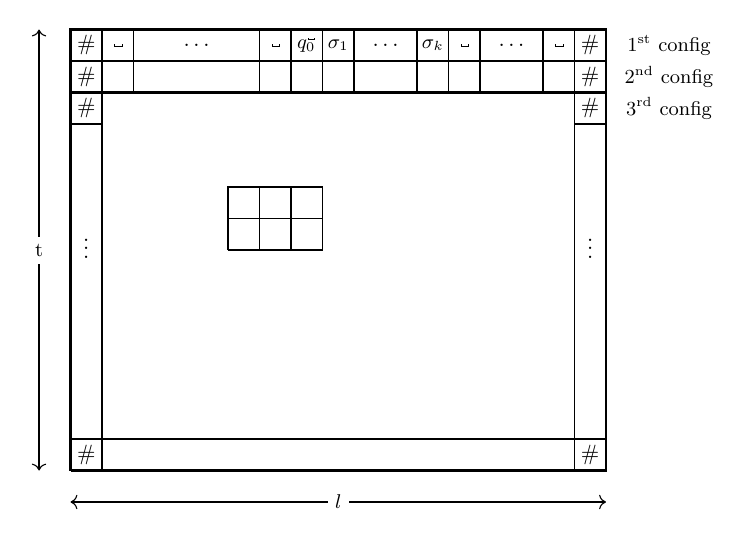
\begin{tikzpicture}[scale=0.8, every node/.style={scale=0.8}]
      \draw[thick] (1.5, -4) -- (1.5, 3) -- (10, 3) -- (10, -4) -- (1.5, -4);
      \draw (2, -4) -- (2, 3);
      \draw (2.5, 3) -- (2.5, 2);
      \draw (9.5, -4) -- (9.5, 3);
      \draw[thick] (1.5, 2.5) -- (10, 2.5);
      \draw[thick] (1.5, -3.5) -- (10, -3.5);
      \draw[thick] (1.5, 2) -- (10, 2);
      \draw[thick] (1.5, 1.5) -- (2, 1.5);
      \draw[thick] (9.5, 1.5) -- (10, 1.5);

      \draw (4.5, 3) -- (4.5, 2);
      \draw (5, 3) -- (5, 2);
      \draw (5.5, 3) -- (5.5, 2);
      \draw (6, 3) -- (6, 2);
      \draw (7, 3) -- (7, 2);
      \draw (7.5, 3) -- (7.5, 2);
      \draw (8, 3) -- (8, 2);
      \draw (9, 3) -- (9, 2);
      %\draw (2.5, 3) -- (2.5, 2);
      %\draw (3, 3) -- (3, 2.5);
      %\draw (4.5, 3) -- (4.5, 2.5);
      %\draw (5, 3) -- (5, 2.5);
      %\draw (5.5, 3) -- (5.5, 2.5);
      %\draw (7.5, 3) -- (7.5, 2.5);

      \node at (1.75, 2.75) {\#};
      \node at (1.75, 2.25) {\#};
      \node at (1.75, 1.75) {\#};
      \node at (1.75, -3.75) {\#};
      \node at (9.75, 2.75) {\#};
      \node at (9.75, 2.25) {\#};
      \node at (9.75, 1.75) {\#};
      \node at (9.75, -3.75) {\#};

      \node at (2.25, 2.75) {\textvisiblespace};
      \node at (3.5, 2.75) {$\ldots$};
      \node at (4.75, 2.75) {\textvisiblespace};
      \node at (5.25, 2.75) {\small $q_0^{\blank}$};
      \node at (5.75, 2.75) {\small $\sigma_1$};
      \node at (6.5, 2.75) {$\ldots$};
      \node at (7.25, 2.75) {\small $\sigma_k$};
      \node at (7.75, 2.75) {\textvisiblespace};
      \node at (8.5, 2.75) {$\ldots$};
      \node at (9.25, 2.75) {\textvisiblespace};

      %\node at (6.5, 2.75) {$\ldots$};
      %\node at (5, 2.25) {$\ldots$};

      \node at (1.75, -0.375) {$\vdots$};
      \node at (9.75, -0.375) {$\vdots$};

      \draw (4, -0.5) -- (4, 0.5) -- (5.5, 0.5) -- (5.5, -0.5) -- (4, -0.5);
      \draw (4.5, -0.5) -- (4.5, 0.5);
      \draw (5, -0.5) -- (5, 0.5);
      \draw (4, 0) -- (5.5, 0);

      \path[<->] (1, -4) edge node[fill=white, anchor=center, pos= 0.5] {\small t} (1, 3);
      \path[<->] (1.5, -4.5) edge node[fill=white, anchor=center, pos=0.5] {\small $l$} (10, -4.5);
      %\path[<->] (5.5, 3.5) edge node[fill=white, anchor=center, pos=0.5] {\small $k$} (7.5, 3.5);

      \node at (11, 2.75) {\small 1\textsuperscript{st} config};
      \node at (11, 2.25) {\small 2\textsuperscript{nd} config};
      \node at (11, 1.75) {\small 3\textsuperscript{rd} config};
    \end{tikzpicture}
  \end{center} 
\end{frame}

\begin{frame}[t]{Configuration String}
  \begin{overlayarea}{\textwidth}{0.08\textwidth}
    %\color{gray}
    \begin{minipage}{0.48\textwidth}
      $\Sigma_{\text{TM}} = \{a, b, c\}$
    \end{minipage}
    \begin{minipage}{0.48\textwidth}
      \onslide<2->{
        \raggedleft
        $\delta(q_1, a) = (q_2, \Some{b}, \textsf{L})$
      }
    \end{minipage}
  \end{overlayarea}
  \begin{overlayarea}{\textwidth}{0.3\textwidth}
    \begin{center}
      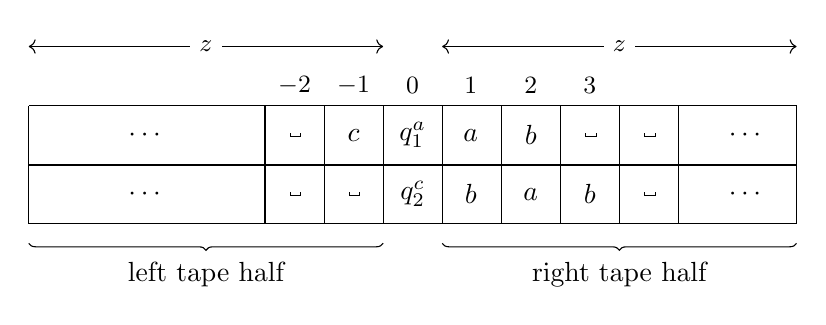
\begin{tikzpicture}
        \draw (0, 0.75) -- (9.75, 0.75);
        \draw (0, 0) -- (9.75, 0);
        \only<2->{
          \draw[thick] (0, 0) -- (9.75, 0);
        }
        \draw (0, 0) -- (0, 0.75);
        \draw (9.75, 0) -- (9.75, 0.75);

        \draw (4.5, 0) -- (4.5, 0.75);
        \draw (5.25, 0) -- (5.25, 0.75);
        \draw (3.75, 0) -- (3.75, 0.75);
        \draw (3, 0) -- (3, 0.75);
        \draw (6, 0) -- (6, 0.75);
        \draw (6.75, 0) -- (6.75, 0.75);
        \draw (7.5, 0) -- (7.5, 0.75);
        \draw (8.25, 0) -- (8.25, 0.75);

        \node at (5.6125, 1) {\small$1$};
        \node at (6.375, 1) {\small$2$};
        \node at (7.125, 1) {\small$3$};
        \node at (4.875, 1) {\small$0$};
        \node at (4.125, 1) {\small$-1$};
        \node at (3.375, 1) {\small$-2$};

        \node at (1.5, 0.375) {$\cdots$};
        \node at (9.125, 0.375) {$\cdots$};
        \node at (5.6125, 0.375) {$a$};
        \node at (6.375, 0.375) {$b$};
        \node at (7.125, 0.375) {\blank};
        \node at (7.875, 0.375) {\blank};
        \node at (4.875, 0.375) {$q_1^a$};
        \node at (4.125, 0.375) {$c$};
        \node at (3.375, 0.375) {\blank};

        \path[<->] (0, 1.5) edge node[fill=white, anchor=center, pos= 0.5] {\small $z$} (4.5, 1.5);
        \node[color=white] at (4.75, 1.5) {l};
        \path[<->] (5.25, 1.5) edge node[fill=white, anchor=center, pos =0.5] {\small $z$} (9.75, 1.5);

        \onslide<2-> {
          \draw (0, -0.75) -- (9.75, -0.75);
          \draw (0, -0.75) -- (0, 0);
          \draw (9.75, -0.75) -- (9.75, 0);

          \draw (4.5, 0) -- (4.5, -0.75);
          \draw (5.25, 0) -- (5.25, -0.75);
          \draw (3.75, 0) -- (3.75, -0.75);
          \draw (3, 0) -- (3, -0.75);
          \draw (6, 0) -- (6, -0.75);
          \draw (6.75, 0) -- (6.75, -0.75);
          \draw (7.5, 0) -- (7.5, -0.75);
          \draw (8.25, 0) -- (8.25, -0.75);

          \node at (1.5, -0.375) {$\cdots$};
          \node at (9.125, -0.375) {$\cdots$};
          \node at (5.6125, -0.375) {$b$};
          \node at (6.375, -0.375) {$a$};
          \node at (7.125, -0.375) {$b$};
          \node at (7.875, -0.375) {\blank};
          \node at (4.875, -0.375) {$q_2^c$};
          \node at (4.125, -0.375) {\blank};
          \node at (3.375, -0.375) {\blank};
        }

        \draw[decorate, decoration={brace, mirror}] (0, -1) -- (4.5, -1) node[midway, yshift=-0.4cm] {left tape half};
        \draw[decorate, decoration={brace, mirror}] (5.25, -1) -- (9.75, -1) node[midway, yshift=-0.4cm] {right tape half};
      \end{tikzpicture}
    \end{center}
  \end{overlayarea}
  \vspace{11ex}
  \emph{special blanks \blank{} for unused regions of the string}
\end{frame}

\begin{frame}[t]{Rewrite Windows: Force Valid Configuration Changes}
  \begin{overlayarea}{\textwidth}{0.08\textwidth}
    %\color{gray}
    \begin{minipage}{0.48\textwidth}
      $\Sigma_{\text{TM}} = \{a, b, c\}$
    \end{minipage}
    \begin{minipage}{0.48\textwidth}
      \onslide<1->{
        \raggedleft
        $\delta(q_1, a) = (q_2, \Some{b}, \textsf{L})$
      }
    \end{minipage}
  \end{overlayarea}
  \begin{overlayarea}{\textwidth}{0.3\textwidth}
    \begin{center}
      \begin{tikzpicture}
        \draw (0, 0.75) -- (9.75, 0.75);
        \draw[thick] (0, 0) -- (9.75, 0);
        \draw (0, 0) -- (0, 0.75);
        \draw (9.75, 0) -- (9.75, 0.75);

        \draw (4.5, 0) -- (4.5, 0.75);
        \draw (5.25, 0) -- (5.25, 0.75);
        \draw (3.75, 0) -- (3.75, 0.75);
        \draw (3, 0) -- (3, 0.75);
        \draw (6, 0) -- (6, 0.75);
        \draw (6.75, 0) -- (6.75, 0.75);
        \draw (7.5, 0) -- (7.5, 0.75);
        \draw (8.25, 0) -- (8.25, 0.75);

        \node at (5.6125, 1) {\small$1$};
        \node at (6.375, 1) {\small$2$};
        \node at (7.125, 1) {\small$3$};
        \node at (4.875, 1) {\small$0$};
        \node at (4.125, 1) {\small$-1$};
        \node at (3.375, 1) {\small$-2$};

        \node at (1.5, 0.375) {$\cdots$};
        \node at (9.125, 0.375) {$\cdots$};
        \node at (5.6125, 0.375) {\only<2-4>{\colorHTwo}$a$};
        \node at (6.375, 0.375) {\only<3-4>{\colorHTwo}$b$};
        \node at (7.125, 0.375) {\only<4>{\colorHTwo}\blank};
        \node at (7.875, 0.375) {\blank};
        \node at (4.875, 0.375) {\only<2-3>{\colorHTwo}$q_1^a$};
        \node at (4.125, 0.375) {\only<2>{\colorHTwo}$c$};
        \node at (3.375, 0.375) {\blank};

        \path[<->] (0, 1.5) edge node[fill=white, anchor=center, pos= 0.5] {\small $z$} (4.5, 1.5);
        \node[color=white] at (4.75, 1.5) {l};
        \path[<->] (5.25, 1.5) edge node[fill=white, anchor=center, pos =0.5] {\small $z$} (9.75, 1.5);

        \draw (0, -0.75) -- (9.75, -0.75);
        \draw (0, -0.75) -- (0, 0);
        \draw (9.75, -0.75) -- (9.75, 0);

        \draw (4.5, 0) -- (4.5, -0.75);
        \draw (5.25, 0) -- (5.25, -0.75);
        \draw (3.75, 0) -- (3.75, -0.75);
        \draw (3, 0) -- (3, -0.75);
        \draw (6, 0) -- (6, -0.75);
        \draw (6.75, 0) -- (6.75, -0.75);
        \draw (7.5, 0) -- (7.5, -0.75);
        \draw (8.25, 0) -- (8.25, -0.75);

        \node at (1.5, -0.375) {$\cdots$};
        \node at (9.125, -0.375) {$\cdots$};
        \node at (5.6125, -0.375) {\only<2-4>{\colorHTwo}$b$};
        \node at (6.375, -0.375) {\only<3-4>{\colorHTwo}$a$};
        \node at (7.125, -0.375) {\only<4>{\colorHTwo}$b$};
        \node at (7.875, -0.375) {\blank};
        \node at (4.875, -0.375) {\only<2-3>{\colorHTwo}$q_2^c$};
        \node at (4.125, -0.375) {\only<2>{\colorHTwo}\blank};
        \node at (3.375, -0.375) {\blank};

        \only<2>{
          \draw[color=\colorTikzC] (4.5, -0.75) -- (4.5, 0.75);
          \draw[color=\colorTikzC] (5.25, -0.75) -- (5.25, 0.75);
          \draw[color=\colorTikzC, thick] (3.75, 0) -- (6, 0);
        }
        \only<3>{
          \draw[color=\colorTikzC] (5.25, -0.75) -- (5.25, 0.75);
          \draw[color=\colorTikzC] (6, -0.75) -- (6, 0.75);
          \draw[color=\colorTikzC, thick] (4.5, 0) -- (6.75, 0);

        }
      \end{tikzpicture}
    \end{center}
  \end{overlayarea}

  \onslide<2->
  \begin{center}
    %\rewwin{\blank & \blank & c}{\blank & \blank & \blank}
    %\rewwin{\blank & c & q_1^a}{\blank & \blank & q_2^c}
    {
      \only<2>{\colorHTwo}
      \trewwin{c}{q_1^a}{a}{\blank}{q_2^c}{b}
    }
    \onslide<3->
    {
      \only<3>{\colorHTwo}
      \trewwin{q_1^a}{a}{b}{q_2^c}{b}{a}
    }
    \onslide<4->
    {
      \only<4>{\colorHTwo}
      \trewwin{a}{b}{\blank}{b}{a}{b}
    }
  \end{center}


\end{frame}

\begin{frame}[t]{Rewrite Rules}
  Add one symbol to the right half of the tape:
    \vspace{-0.5ex}
      \begin{center}
        \begin{tikzpicture}
          \draw (5.25, 0.75) -- (9.75, 0.75);
          \draw[thick] (5.25, 0) -- (9.75, 0);
          \draw (5.25, 0) -- (5.25, 0.75);
          \draw (9.75, 0) -- (9.75, 0.75);

          \draw (5.25, 0) -- (5.25, 0.75);
          \draw (6, 0) -- (6, 0.75);
          \draw (6.75, 0) -- (6.75, 0.75);
          \draw (7.5, 0) -- (7.5, 0.75);
          \draw (8.25, 0) -- (8.25, 0.75);

          \node at (9.125, 0.375) {$\cdots$};
          \node at (7.125, 0.375) {\blank};
          \node at (7.875, 0.375) {\blank};
          \only<1>{
            \node at (5.6125, 0.375) {$a$};
            \node at (6.375, 0.375) {$b$};
          }
          \only<2->{ 
            \node at (5.6125, 0.375) {$\sigma_1$};
            \node at (6.375, 0.375) {$\sigma_2$};
          }


          \draw (5.25, -0.75) -- (9.75, -0.75);
          \draw (5.25, -0.75) -- (5.25, 0);
          \draw (9.75, -0.75) -- (9.75, 0);

          \draw (5.25, 0) -- (5.25, -0.75);
          \draw (6, 0) -- (6, -0.75);
          \draw (6.75, 0) -- (6.75, -0.75);
          \draw (7.5, 0) -- (7.5, -0.75);
          \draw (8.25, 0) -- (8.25, -0.75);

          \node at (9.125, -0.375) {$\cdots$};
          \node at (7.875, -0.375) {$\blank$};
          \only<1>{
            \node at (5.6125, -0.375) {$b$};
            \node at (6.375, -0.375) {$a$};
            \node at (7.125, -0.375) {$b$};
          }
          \only<2->{
            \node at (5.6125, -0.375) {$\sigma_3$};
            \node at (6.375, -0.375) {$\sigma_1$};
            \node at (7.125, -0.375) {$\sigma_2$};
          }
        \end{tikzpicture}
        \end{center}
      \onslide<2->{
        \begin{center}
          $\sigma_i \in \Sigma_{\text{TM}}$
        \end{center}
      }

      \begin{center}
        \trewwin{\only<1>{a}\only<2->{\sigma_1}}{\only<1>{b}\only<2->{\sigma_2}}{\blank}{\only<1>{b}\only<2->{\sigma_3}}{\only<1>{a}\only<2->{\sigma_1}}{\only<1>{b}\only<2->{\sigma_2}}
        \onslide<3->{
          \trewwin{\sigma_2}{\blank}{\blank}{\sigma_1}{\sigma_2}{\blank}
          \trewwin{\blank}{\blank}{\blank}{\sigma_2}{\blank}{\blank}
          \vfill{}$\cdots$\vfill{}
        }
      \end{center}
\end{frame}

\begin{frame}{Parallel Rewriting (\PR{})}
  \only<2->{\frametitle{Explicit Representation of Turing machines}}
  Given: 
  \begin{itemize}
    \item an initial string $x_0 \in \Sigma^l$ over an alphabet $\Sigma$ \\
      \onslide<2->{{\color{blue}{\emph{representation of initial config}}}}
    \item a set of rewrite windows $R$ of width $w$ \\ 
      \onslide<2->{{\color{blue}{\emph{possible local behaviours of the Turing machine}}}}
    \item a step count $t$ \\
      \onslide<2->{{\color{blue}\emph{number of TM steps}}}
    \item a set of final substring constraints $\Rfinal$ \\
      \onslide<2->{{\color{blue}\emph{symbols of accepting states}}}
  \end{itemize}
  Determine: $\exists$ $x_1, \ldots, x_t \in \Sigma^l$ s.t.\ 
  \begin{itemize}
    \item $x_i \rightsquigarrow x_{i+1}$: ``for all offsets, there exists a rewrite window''
    \item there exists an element $x \in R_{\mathit{final}}$ which is a substring of $x_t$
  \end{itemize}
\end{frame}

\begin{frame}{Nondeterministic Input}
  \begin{itemize}
    \item ``Guess'' certificate of length $\le k'$ with a single rewrite step
    \item Add symbols $\{\underline{\#}, \underline{\blank}, \underline{*}, \underline{q^{\blank}}, \underline{\sigma}\}$ for initial state $q$ and $\sigma : \Sigma$
  \end{itemize}

  \vspace{2ex}
  Initial string: 
  \begin{center}
  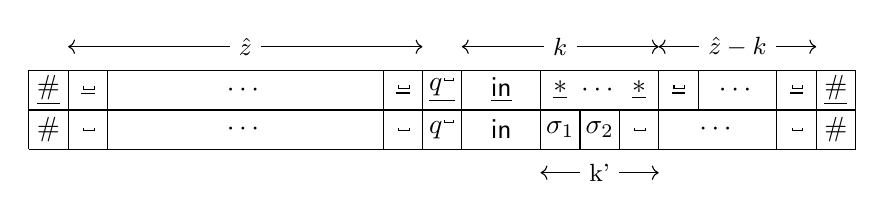
\begin{tikzpicture}[scale=1.0]
    \draw (0, 0.5) -- (10.5, 0.5);
    \draw[thick] (0, 0) -- (10.5, 0);
    \draw (0, 0) -- (0, 0.5);
    \draw (10.5, 0) -- (10.5, 0.5);

    \draw (0.5, 0.5) -- (0.5, 0);
    \draw (1, 0.5) -- (1, 0);
    \draw (10, 0.5) -- (10, 0);
    \draw (9.5, 0.5) -- (9.5, 0);
    \draw (5, 0.5) -- (5, 0);
    \draw (5.5, 0.5) -- (5.5, 0);
    \draw (4.5, 0.5) -- (4.5, 0);
    %\draw (6, 0.5) -- (6, 0);
    \draw (6.5, 0.5) -- (6.5, 0);
    %\draw (7, 0.5) -- (7, 0);
    %\draw (7.5, 0.5) -- (7.5, 0);
    \draw (8, 0.5) -- (8, 0);
    \draw (8.5, 0.5) -- (8.5, 0);

    \node at (9, 0.25) {$\cdots$};
    \node at (7.25, 0.25) {$\cdots$};
    \node at (2.75, 0.25) {$\cdots$};

    \node at (0.25, 0.25) {\underline{\#}};
    \node at (0.75, 0.24) {$\underline{\blank}$};
    \node at (4.75, 0.25) {$\underline{\blank}$};
    \node at (5.25, 0.25) {$\underline{q^{\blank}}$};
    \node at (6, 0.25) {\underline{\textsf{in}}};
    \node at (6.75, 0.25) {$\underline{*}$};
    \node at (7.75, 0.25) {$\underline{*}$};
    \node at (8.25, 0.25) {$\underline{\blank}$};
    \node at (9.75, 0.25) {$\underline{\blank}$};
    \node at (10.25, 0.25) {\underline{\#}};

    \draw (0, -0.5) -- (10.5, -0.5);
    \draw (0, 0) -- (0, -0.5);
    \draw (10.5, 0) -- (10.5, -0.5);

    \draw (0.5, -0.5) -- (0.5, 0);
    \draw (1, -0.5) -- (1, 0);
    \draw (10, -0.5) -- (10, 0);
    \draw (9.5, -0.5) -- (9.5, 0);
    \draw (5, -0.5) -- (5, 0);
    \draw (5.5, -0.5) -- (5.5, 0);
    \draw (4.5, -0.5) -- (4.5, 0);
    %\draw (6, -0.5) -- (6, 0);
    \draw (6.5, -0.5) -- (6.5, 0);
    \draw (7, -0.5) -- (7, 0);
    \draw (7.5, -0.5) -- (7.5, 0);
    \draw (8, -0.5) -- (8, 0);
    %\draw (7.5, -0.5) -- (7.5, 0);
    %\draw (8, -0.5) -- (8, 0);
    %\draw (8.5, -0.5) -- (8.5, 0);

    \node at (2.75, -0.25) {$\cdots$};
    \node at (0.25, -0.25) {\#};
    \node at (0.75, -0.25) {\blank};
    \node at (4.75, -0.25) {\blank};
    \node at (5.25, -0.25) {$q^{\blank}$};
    \node at (6, -0.25) {\textsf{in}};
    \node at (6.75, -0.25) {$\sigma_1$};
    \node at (7.25, -0.25) {$\sigma_2$};
    \node at (7.75, -0.25) {\blank};
    \node at (8.75, -0.25) {$\cdots$};
    \node at (9.75, -0.25) {\blank};
    \node at (10.25, -0.25) {\#};

    \path[<->] (5.5, 0.8) edge node[fill=white, anchor=center, pos= 0.5] {\small $k$} (8, 0.8);
    \path[<->] (0.5, 0.8) edge node [fill = white, anchor=center, pos=0.5] {\small $\hat{z}$} (5, 0.8);
    \path[<->] (8, 0.8) edge node [fill = white, anchor =center, pos=0.5] {\small $\hat{z}-k$} (10, 0.8);
    \path[<->] (6.5, -0.8) edge node[fill =white, anchor = center, pos = 0.5] {\small{k'}} (8, -0.8);
  \end{tikzpicture}
\end{center}
\end{frame}

\section{Encoding as CNF}

\begin{frame}<1-2>[label=chain]{Chain of Reductions}
  \begin{center}
    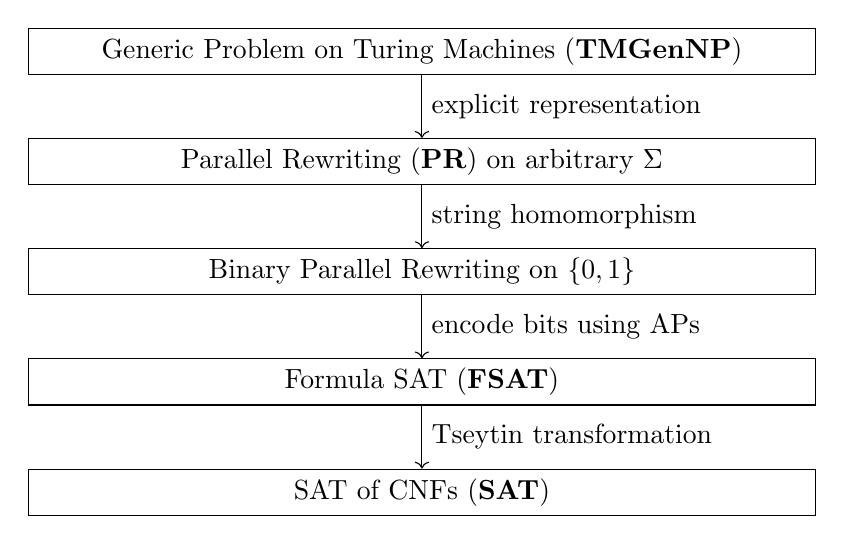
\begin{tikzpicture}[scale=1, every node/.style={scale=1}, node distance = 0.8cm]
      \node[rectangle, draw=black, minimum width=10cm] (gennp) {Generic Problem on Turing Machines (\gennp{})}; 
      \node[rectangle, draw=black, minimum width = 10cm, below = of gennp] (strrew1) {Parallel Rewriting (\PR{}) on arbitrary $\Sigma$};
      \draw[->] 
        (gennp) edge node[right] {explicit representation} (strrew1);

      \onslide<2->{ 
        \node[rectangle, draw=black, below = of strrew1, minimum width = 10cm] (strrew2) {Binary Parallel Rewriting on $\{0, 1\}$};
        \draw[->] 
          (strrew1) edge node[right] {string homomorphism} (strrew2);
      }
      \onslide<3->{
        \node[rectangle, draw=black, below = of strrew2, minimum width = 10cm] (csat) {Formula SAT (\fsat{})};
        \draw[->] 
         (strrew2) edge node[right] {encode bits using APs} (csat);

      }
      \onslide<4->{
        \node[rectangle, draw=black, below = of csat, minimum width = 10cm] (sat) {SAT of CNFs (\sat{})};
        \draw[->] 
          (csat) edge node[right] {Tseytin transformation} (sat);
      }
    \end{tikzpicture}
  \end{center}

\end{frame}

\begin{frame}{To a Binary Alphabet}
  \begin{itemize}
    \item arbitrary alphabet $\Sigma = \{\sigma_0, \ldots, \sigma_{\length{\Sigma} -1} \}$
    \item string homomorphism $h : \Sigma^* \rightarrow {\{0, 1\}}^*$ 
      \[\sigma_i \mapsto 0^i 1 0^{\length{\Sigma} - i - 1} \]
    \item in general: injective \emph{uniform} homomorphisms \\
      $\rightarrow$ scale length up by constant factor
  \end{itemize}
\end{frame}

\againframe<3>{chain}

\newcommand{\defeq}{\coloneqq}
\newcommand{\bvar}{\textsf{var}}
\newcommand{\formula}{\mathcal{F}}
\newcommand{\encodesPred}{\textsf{encodesPredAt}}

\begin{frame}{Encoding as a Boolean Formula}
  \begin{itemize}
    \item $f : \formula \defeq \btrue \bnfmid v \bnfmid f_1 \lor f_2 \bnfmid f_1 \land f_2 \bnfmid \lnot f \qquad (v : \nat)$
    \item explicit assignments $e : \listsof{\bool}$ to variables $[s, s + \length{e})$
    \item encoding of predicates $p : \listsof{\bool} \rightarrow \Prop$: \[\encodesPred~\textsf{start}~l~f~p \defeq \forall a, a \models f \leftrightarrow p~(a[\textsf{start}, \textsf{start} + l])\]
    \item $\textsf{encodeBit}~\textsf{var}~\textsf{bit} \defeq \ITE{\textsf{bit}}{\textsf{var}}{\lnot \textsf{var}}$
      \[\encodesPred~v~1~(\textsf{encodeBit}~v~b) (\lambda e. e = [s]) \]
    \item $\Phi \defeq \Phi_{\textsf{init}} \land \Phi_{\textsf{trans}} \land \Phi_{\textsf{final}}$
      \begin{align*}
        \Phi_{\textsf{trans}} \defeq \bigwedge_{\text{lines}} \bigwedge_{\text{positions}} \bigvee_{w \in R} \bigwedge_{\text{characters of } w} \textsf{encodeBit}
      \end{align*}
  \end{itemize} 
\end{frame}

\againframe<4>{chain}

\begin{frame}{The Tseytin Transformation}
  Goal: translation into CNF ($\bigwedge_{C \in \textsf{clauses}} \bigvee_{l \in \textsf{literals}(C)} l$)
  \TODO{todo}
    %\item naive approach: exponential blowup
    %\item Tseytin: introduce new variables for each subformula
  %\end{itemize}
\end{frame}

\section{Conclusion}
\newcommand{\redP}{\ensuremath{\preceq_p}}
\newcommand{\Clique}{\normalfont\textbf{Clique}}
\begin{frame}{Contributions}
  \begin{block}{Main result}
    If \gennp{} is \NP{}-hard, then \SAT{} is \NP{}-complete. 
  \end{block}
  \begin{itemize}
    \item factorisation of the textbook proof~\cite{Sipser:TheoryofComputation} to make mechanisation feasible: new \PR{} problem
    \item full running-time analysis in L
  \end{itemize}

  Moreover: 
  \begin{itemize}
    \item reduction $\text{$k$-\SAT{}} \redP{} \Clique{}$
    \item conditional \NP{}-completeness of $\Clique{}$
    \item $\gennp{} \in \NP{}$
    \item formalisation of $\#P$
  \end{itemize}
\end{frame}

\begin{frame}{Future Work}
  \begin{itemize}
    \item missing reduction from L to \gennp{} 
    \item space-related results, e.g.\ Savitch
    \item nondeterministic L
    \item complexity theory beyond decision problems?
    \item binary encodings
  \end{itemize}
\end{frame}

\miniframesoff
\section{}

\begin{frame}{LOC}
\end{frame}

\begin{frame}{Comparison with~\cite{gamboa:cook}}

\end{frame}

\begin{frame}{Representation Relations}
\end{frame}

\begin{frame}{Simulation Proof}
\end{frame}

\begin{frame}{Tseytin: Correctness Relation}
\end{frame}

\begin{frame}{Some Rewrite Rules}
\end{frame}

\begin{frame}{possible other stuff}
  \begin{itemize}
    \item 2-PR vs 3-PR
    \item polarities and motivation for them
    \item procedure for proving rt bounds
  \end{itemize}
\end{frame}

\begin{frame}[allowframebreaks]{References}
  \nocite{Sipser:TheoryofComputation}
  \nocite{Bläser:TISkript}
  \bibliographystyle{apalike}
  \bibliography{references}{}
\end{frame}
\end{document}
